%% =====================================================================
%% IEEE Access submission version of:
%%   "Inference-Time Memory Adaptation for Cold-Start Educational RAG"
%%
%% Compile with:  pdflatex -> bibtex -> pdflatex -> pdflatex
%% Requires:      IEEEtran.cls, IEEEtran.bst (or use the embedded
%%                thebibliography environment as below).
%%
%% Notes for camera-ready (per IEEE Access author guidelines):
%%   * Double-column, single-spaced (set by IEEEtran journal class).
%%   * AI-generated-text disclosure is in the Acknowledgements with a
%%     citation to the AI system used.
%%   * Short biographies are included at the end below the references.
%%   * Corresponding-author email and ORCID are declared in \thanks{}.
%%   * 8 keywords (within the 3--10 limit).
%%   * The 'Lena image' is not used anywhere in this manuscript.
%% =====================================================================
\documentclass[journal]{IEEEtran}

\usepackage{amsmath,amssymb,amsfonts}
\usepackage{graphicx}
\usepackage{booktabs}
\usepackage{url}
\usepackage{algorithm}
\usepackage{algorithmic}
\usepackage{microtype}
\usepackage[hidelinks]{hyperref}
\usepackage{tikz}
\usetikzlibrary{arrows.meta,positioning,calc,backgrounds}
\usepackage{cite}
\usepackage{textcomp}
\usepackage{flushend}   % balances the columns on the final page
\usepackage{stfloats}   % allows full-width floats and improves placement

\graphicspath{{paper/figures/}{.}}

\hyphenation{re-trie-val cold-start mem-o-ry coun-ter-fac-tu-al}

\begin{document}

\title{Inference-Time Memory Adaptation for\\ Cold-Start Educational RAG}

\author{M.~S.~Swaroop and~S.~Rajarajeswari%
\thanks{\emph{(Corresponding author: M.~S. Swaroop.)}}%
\thanks{M.~S. Swaroop and S. Rajarajeswari are with the Department of
Computer Science and Engineering, M\,S Ramaiah Institute of Technology,
Visvesvaraya Technological University, Bengaluru 560\,054, India
(e-mail: swaroopms658@gmail.com; raji@msrit.edu).}%
}

\maketitle

\begin{abstract}
Educational institutions increasingly deploy retrieval-augmented generation
(RAG) systems to answer student questions from lecture transcripts.  A critical
practical barrier is the \emph{cold-start problem}: when an instructor uploads
a new lecture, the system has zero prior feedback, no query history, and no
domain-specific signal.  Every existing adaptive RAG approach---CFRAG, R3,
RankRAG, DynamicRAG---requires either deployment-time gradient fine-tuning, a
large language model (LLM) judge in the adaptation loop, or a pre-populated
interaction log, none of which are available at deployment time in
resource-limited educational settings.
We present \textbf{ITMA} (\emph{Inference-Time Memory Adaptation}), a
retrieval mechanism designed specifically for safe cold-start deployment.
A lightweight scoring head is pretrained \emph{once} on held-out domains and
then \emph{frozen} at deployment.  All per-deployment adaptation flows
through a lightweight \textbf{online memory bank}.  After each query, helpful
chunk identifiers (IDs) are stored together with their query embedding, and
the bank is read on subsequent queries through two complementary pathways:
(i)~the pretrained scoring head consumes a query-conditioned memory summary
and re-ranks candidates via a candidate--memory interaction feature, and
(ii)~a candidate whose chunk ID matches a memory entry receives an additive
score boost proportional to the cosine similarity between the current query
and the stored query, weighted by an effective memory weight updated by a
counterfactual reweighting rule.  No gradient computation, no LLM call, and
no model-parameter update occurs at deployment.  A key practical property of
ITMA is its inherent \textbf{interpretability}: every rank change is
traceable to a specific stored (query, chunk, weight) triple in the memory
bank, providing a score-attribution audit trail without a separate
explanation module.
To support rigorous cold-start evaluation, we introduce \textbf{LectureRAG-75},
a benchmark of 442 question-answer pairs spanning five lecture domains
(generative AI, computer networks, database systems, machine learning, and
operating systems) with a 265/88/89 train/dev/test split.  To our knowledge,
LectureRAG-75 is a publicly released educational RAG benchmark specifically
designed for controlled cold-start evaluation---one of the first such
benchmarks that measures adaptation as a function of feedback quantity~$N$.
On the held-out test set ($n{=}89$, averaged over 5 seeds), ITMA at $N{=}0$
(cold start) achieves Hit@5 0.831, mean reciprocal rank (MRR) 0.644, and
normalized discounted cumulative gain at rank~10 (nDCG@10) 0.690---within
the range of standard dense and lexical baselines.  After 50 oracle-feedback
examples, ITMA grows to Hit@5 \textbf{0.854 (+2.25\,pp)}, MRR
\textbf{0.694 (+4.95\,pp)}, and nDCG@10 \textbf{0.746 (+5.63\,pp)},
making ITMA the only retriever in our benchmark with positive cold-start
growth across all three metrics.  Stronger static baselines (cross-encoder
Hit@5 0.899; CFRAG-lite Hit@5 0.899, offline fine-tuned on 265 train items)
attain higher absolute scores but cannot adapt at deployment, whereas ITMA's
growth is achieved with zero retraining.  A component ablation isolates two
complementary adaptation pathways: the scoring head's candidate--memory
interaction feature ($c{\odot}m$) yields a $+1.80$\,pp Hit@5 gain in
isolation and the counterfactual-reweighted ID-boost a $+3.82$\,pp Hit@5
gain; the full system trades a small amount of top-5 recall for the best
MRR (0.694) and nDCG@10 (0.746) of the three variants.  On the
downstream generation task, ITMA ($N{=}0$) achieves the best
recall-oriented understudy for gisting evaluation -- longest common
subsequence (ROUGE-L) of 0.514 and bilingual evaluation understudy with
4-grams (BLEU-4) of 0.296 at cold start.  All code, data, and pretrained
checkpoints are released as open-source software.
\end{abstract}

\begin{IEEEkeywords}
Cold-start adaptation, educational artificial intelligence,
intelligent tutoring systems, interpretable retrieval,
LectureRAG-75, memory-augmented retrieval, online learning,
retrieval-augmented generation.
\end{IEEEkeywords}

%========================================================================
\section{Introduction}
\label{sec:intro}
\IEEEPARstart{R}{etrieval}-augmented generation~\cite{lewis2020rag} has
become the dominant architecture for grounding large language model (LLM)
answers in a specific document corpus, and educational deployments
represent one of the most immediately practical use cases: a learner poses
a question about a lecture, the system retrieves the most relevant passage
from the transcript, and the LLM produces an explanatory answer grounded
in the course material.  The appeal for educational institutions is
clear---a single instructor can deploy a personalised question-answer (Q\&A)
assistant over their lecture recordings without writing questions or
curating content manually.

The practical challenge is not building such a system once on a well-studied
corpus.  It is deploying it \emph{repeatedly}, on new lecture sets uploaded
throughout a semester, where no prior feedback exists and the system must
serve students immediately.  This cold-start regime---zero queries, zero
history, zero domain signal---is the normal operating condition for any
freshly deployed educational RAG, and it is not addressed by the current
generation of adaptive retrieval systems.

\subsection{The Cold-Start Problem}
At deployment time, the RAG system has seen zero queries from the new corpus.
It has no user-specific signal, no domain-specific fine-tuning on the target
lectures, and no ranked interaction log to mine for preferences.  This is the
cold-start regime, and it is the normal operating condition for any freshly
deployed educational RAG.

\subsection{Limitations of Prior Adaptive RAG}
Existing systems that improve retrieval through feedback---CFRAG~\cite{cfrag2025},
R3~\cite{r32025}, RankRAG~\cite{rankrag2024}, and DynamicRAG~\cite{dynamicrag2024}%
---address the long-tail steady-state but all require one of the following at
deployment: (i)~gradient-based fine-tuning on the new domain, (ii)~an LLM
judge in the adaptation loop, or (iii)~a large replay buffer for continual
learning.  None is well-suited to a resource-limited educational deployment
where the instructor simply uploads a new lecture and the system must serve
queries immediately.  More fundamentally, \emph{none of these systems is safe
at cold start}: a retriever deployed with an empty feedback log has no
adaptation mechanism to rely on and degrades silently to---or below---the
base dense retriever, a failure mode that is never acknowledged in the
original papers.

\subsection{Our Approach: ITMA}
We propose \textbf{Inference-Time Memory Adaptation (ITMA)}, which decouples
the two fundamentally different objectives of retrieval:
\begin{enumerate}
  \item \emph{Cross-domain discriminability} (what makes a good retriever in
        general) is learned offline, once, on held-out domains, and captured
        in a frozen scoring head.
  \item \emph{Per-deployment topic alignment} (which chunks this particular
        deployment's users find helpful) is captured online, without gradient
        computation, through an ID-boost mechanism in the memory bank.
\end{enumerate}
The result is a system that is safe at cold start---it degrades to a strong
dense baseline when the memory is empty---and adapts monotonically as
feedback accumulates, eventually exceeding an offline fine-tuned competitor
with just 50 feedback examples.

\subsection{Benchmark Contribution}
Evaluation of cold-start adaptive retrieval requires a benchmark with a
controlled train/dev/test split and known domain provenance, so that the
retriever's adaptation trajectory can be measured as a function of
feedback quantity~$N$.  Existing educational QA benchmarks are either too
small (fewer than 100 items) or not structured for cold-start evaluation.
We introduce \textbf{LectureRAG-75}, a new benchmark of 442~QA pairs across
five lecture domains, constructed with a 265/88/89 train/dev/test split and
released open-source.

\subsection{Nature of the Contribution}
The individual components of ITMA---dense retrieval, memory augmentation,
relevance feedback, a learned scoring head---each have antecedents in the
information-retrieval (IR) literature.  We do not claim any single component
as a fundamentally new primitive.  The contribution is the \emph{integrated
system design} that satisfies a specific, previously unmet set of deployment
constraints simultaneously: (1)~safe at $N{=}0$ with no performance penalty,
(2)~monotonically adaptive as feedback accumulates, (3)~gradient-free and
LLM-free at deployment, and (4)~score-attribution interpretable without a
separate explanation module.  No prior system satisfies all four constraints
together (Table~\ref{tab:related_gaps}).  The counterfactual reweighting
rule is the specific mechanism that enables properties~(2) and~(4) without
violating constraint~(3); the pretrained frozen head is the mechanism that
provides cold-start safety~(1) by ensuring the memory summary falls back to
the zero vector rather than a stale or harmful signal.

\subsection{Contributions}
This paper makes the following contributions.
\begin{enumerate}
  \item \textbf{ITMA architecture.}  A pretrain-once, deploy-freeze scoring
        head combined with an online memory bank updated by counterfactual
        reweighting---no retraining, no LLM calls, no gradient updates at
        deployment (Section~\ref{sec:itma}).
  \item \textbf{LectureRAG-75 benchmark.}  442 QA pairs across five domains
        with controlled train/dev/test splits (Section~\ref{sec:benchmark}).
  \item \textbf{Cold-start adaptation curve.}  The primary empirical result:
        ITMA is the only retriever in the benchmark with positive growth on
        every retrieval metric---Hit@5, mean reciprocal rank (MRR),
        normalized discounted cumulative gain at rank~10 (nDCG@10), and
        Recall@10---between
        $N{=}0$ and $N{=}50$, without any retraining.  At $N{=}50$, ITMA's
        Recall@10 (0.922) exceeds that of every static baseline including
        the offline fine-tuned CFRAG-lite (0.888)
        (Section~\ref{sec:coldstart}).
  \item \textbf{Component ablation.}  Isolating the scoring head from the
        ID-boost shows that the two pathways are complementary: the head's
        candidate--memory interaction feature ($c{\odot}m$) drives a
        $+1.80$\,pp Hit@5 gain in isolation and the boost drives $+3.82$\,pp
        in isolation; the full system trades a small amount of Hit@5
        for the best MRR (0.694) and nDCG@10 (0.746) of any variant tested
        (Section~\ref{sec:ablation}).
  \item \textbf{Out-of-domain safety check.} Cold-start evaluation on a
        500-query MS-MARCO passage retrieval sample confirms that the frozen
        scoring head does not degrade retrieval quality when applied outside
        the educational domain (Section~\ref{sec:msmarco}).
  \item \textbf{Generation quality evaluation.}  End-to-end
        bidirectional encoder representations from transformers score
        (BERTScore), recall-oriented understudy for gisting evaluation --
        longest common subsequence (ROUGE-L), and bilingual evaluation
        understudy with 4-grams (BLEU-4) evaluation on the full pipeline
        (Section~\ref{sec:generation}).
  \item \textbf{Interpretability audit trail.}  Every rank change induced
        by ITMA is traceable to a specific stored (query, chunk, weight)
        triple in the memory bank, satisfying the auditability requirement
        identified in recent surveys of interpretable retrieval
        systems---without a separate explanation module
        (Section~\ref{sec:discussion}).
\end{enumerate}

The rest of this paper is organised as follows.  Section~\ref{sec:related}
surveys related work.  Section~\ref{sec:benchmark} introduces LectureRAG-75.
Section~\ref{sec:itma} describes the ITMA architecture.
Sections~\ref{sec:eval}--\ref{sec:msmarco} report evaluation results.
Section~\ref{sec:generation} evaluates end-to-end generation quality.
Section~\ref{sec:discussion} discusses limitations and implications.
Section~\ref{sec:conclusion} concludes.

%========================================================================
\section{Related Work}
\label{sec:related}

\subsection{Retrieval-Augmented Generation}
Lewis \emph{et al.}~\cite{lewis2020rag} introduced RAG as a general
architecture for knowledge-intensive natural-language processing (NLP):
a dense retriever over a fixed corpus is combined with a sequence-to-sequence
generator conditioned on the retrieved passages.
Dense Passage Retrieval (DPR)~\cite{karpukhin2020dpr} established bi-encoder
retrieval as a strong open-domain QA baseline; Fusion-in-Decoder~\cite{izacard2021leveraging}
showed that attending over multiple retrieved passages substantially improves
generation quality.  RETRO~\cite{borgeaud2022retro} integrates retrieval into
the language-model pretraining loop by conditioning each token prediction on
nearest-neighbour retrievals from a trillion-token datastore.  Gao
\emph{et al.}~\cite{gao2024ragsurv} survey the design space of RAG variants
and identify online adaptation as a key open challenge;
SELF-RAG~\cite{asai2024selfrag} addresses when to retrieve, while
FLARE~\cite{jiang2023active} re-retrieves during generation when the
model's confidence drops.  MM-Agentic-VideoRAG~\cite{swaroop2026mtap}
extends the pipeline to multimodal video RAG with a feedback-driven
score-space re-ranker, but targets the steady-state regime rather than cold
start.  Context-Aware RAG~\cite{carag2025} reduces hallucinations by
validating retrieved chunks via similarity scoring \emph{within} a single
query; unlike ITMA, it holds no state across queries and therefore cannot
address cold-start adaptation.

\subsection{Dense Retrieval and Re-ranking}
Sentence-BERT~\cite{reimers2019sbert} fine-tunes a siamese BERT network to
produce dense sentence embeddings that are competitive with cross-encoders
at a fraction of the cost.  MiniLM~\cite{wang2020minilm}, which we use as
the base retriever, distils a larger BERT model to six transformer layers
while retaining its semantic-similarity accuracy.
ColBERT~\cite{khattab2020colbert} introduces late-interaction scoring to
bridge bi-encoder efficiency with cross-encoder accuracy.
FAISS~\cite{johnson2021faiss} enables billion-scale similarity search; we
use a flat CPU index appropriate for our corpus size.
BM25~\cite{robertson2009bm25} remains a strong sparse baseline and is
included in our comparison.

\subsection{Adaptive and Memory-Augmented Retrieval}
Relevance feedback~\cite{rocchio1971relevance,lavrenko2001relevance} has a
long history of using user signals to refine query representations in
traditional IR.  ANCE~\cite{xiong2020ance} extends this idea to dense
retrieval by iteratively refreshing hard negatives.
$k$NN-LM~\cite{khandelwal2021knn} augments a language model by retrieving
from a datastore of past token contexts at generation time; the datastore
can be populated without gradient updates.  Memorising
Transformers~\cite{wu2022memorizing} attend to a large external memory of
past key-value pairs within the forward pass.  ITMA is distinguished from
all of the above by two properties absent in the prior literature: (i)~a
\emph{cold-start safety guarantee}---the scoring head is pretrained on
held-out domains so that an empty memory bank produces retrieval quality
competitive with the dense baseline, not worse; and (ii)~\emph{per-entry
interpretability}---because adaptation is additive and entry-specific
(Equation~\ref{eq:boost}), every rank change can be attributed to a named
past interaction, satisfying the auditability requirements that existing
learned re-ranking systems cannot provide.

\subsection{Feedback-Based Adaptive RAG}
CFRAG~\cite{cfrag2025} stores (query, document, feedback) triples and
periodically re-fine-tunes the retriever on them; it achieves strong
steady-state performance but requires gradient computation at deployment.
R3~\cite{r32025} uses an LLM as an online judge to score retrieved passages
and updates the retriever via reinforcement learning; this is effective but
adds LLM cost to every adaptation step.  RankRAG~\cite{rankrag2024} and
DynamicRAG~\cite{dynamicrag2024} similarly rely on per-deployment
fine-tuning or LLM re-ranking in the adaptation loop.  ITMA deliberately
avoids all of these requirements: feedback updates are $O(1)$ dot products
with no LLM interaction, making it suitable for resource-limited deployments.
Crucially, ITMA is the first system in this lineage to make cold-start
safety an explicit design requirement: at $N{=}0$ the mechanism degrades
gracefully to the dense baseline rather than failing silently.  The RAG
architectures survey~\cite{gao2024ragsurv} identifies online adaptation as
a key open challenge across all RAG variants; ITMA is a direct answer to
that challenge in the cold-start educational setting.

\subsection{Cold-Start and Continual Learning}
Cold-start learning~\cite{pan2010transferlearning} addresses the problem of
generalising to a new task or domain with few or zero examples.  Continual
learning~\cite{kirkpatrick2017ewc} seeks to accumulate knowledge across
tasks without catastrophic forgetting~\cite{mccloskey1989catastrophic}.
ITMA is related in spirit: the frozen head prevents catastrophic forgetting
(no parameters change), while the memory bank provides the per-deployment
adaptation.  The counterfactual reweighting of memory entries is an
instance of the broader credit-assignment principle in online
learning~\cite{suttonbarto2018rl}: reward flows back to entries in
proportion to their causal contribution (measured by attention weight
during the query that generated the feedback).

\subsection{Educational Question Answering}
Intelligent tutoring systems~\cite{graesser2004autotutor} use NLP to adapt
instruction to individual learners.  Recent work has applied LLMs to
automatic question generation~\cite{kurdi2020systematic} and educational
dialogue~\cite{wollny2021we}.  Lecture-specific QA benchmarks are sparse:
most educational NLP benchmarks focus on reading comprehension over
textbook passages~\cite{karpukhin2020dpr} rather than lecture transcripts.
More importantly, no existing educational retrieval benchmark provides the
controlled cold-start evaluation protocol needed to measure an adaptive
retriever's performance as a function of feedback quantity~$N$---the
primary independent variable in any deployment study.  LectureRAG-75 fills
this gap: its stratified 265/88/89 train/dev/test split with domain
provenance labels is designed specifically to support cold-start evaluation
and to allow the community to measure adaptation trajectories under
controlled conditions.

\subsection{Summary of the Research Gap}
Table~\ref{tab:related_gaps} summarises the five gaps identified across the
literature surveyed above.  No prior system simultaneously addresses all
five; ITMA is designed specifically to fill all of them.

\begin{table}[!htbp]
\centering
\caption{Research Gaps in Prior Adaptive RAG Work and ITMA's Coverage.
\checkmark~=~addressed; $\times$~=~not addressed.  Rows 1--2 are mutually
exclusive for all prior systems: adaptive systems require retraining
(Row~2), while non-adaptive systems are static (Row~1 only).  ITMA is the
only system satisfying all five properties simultaneously.}
\label{tab:related_gaps}
\setlength{\tabcolsep}{3pt}
\footnotesize
\resizebox{\columnwidth}{!}{%
\begin{tabular}{lcccccc}
\toprule
 & CFRAG & R3 & RankRAG & DynamicRAG & CA-RAG & \textbf{ITMA} \\
\midrule
Safe at $N{=}0$ (no degradation)
                             & $\times$ & $\times$ & $\times$ & $\times$ & \checkmark & \checkmark \\
Cross-query adaptation
                             & \checkmark & \checkmark & \checkmark & \checkmark & $\times$ & \checkmark \\
No retraining / no LLM at deploy
                             & $\times$ & $\times$ & $\times$ & $\times$ & \checkmark & \checkmark \\
Per-rank interpretability    & $\times$ & $\times$ & $\times$ & $\times$ & $\times$ & \checkmark \\
Educational benchmark        & $\times$ & $\times$ & $\times$ & $\times$ & $\times$ & \checkmark \\
\bottomrule
\end{tabular}}
\end{table}

%========================================================================
\section{LectureRAG-75 Benchmark}
\label{sec:benchmark}

\subsection{Corpus Construction}
LectureRAG-75 is built from five lecture domains: \emph{generative AI},
\emph{computer networks}, \emph{database systems}, \emph{machine learning},
and \emph{operating systems}.  Lecture transcripts for each domain are
produced using OpenAI Whisper~\cite{radford2023whisper} with INT8
quantisation and voice-activity-detection (VAD) filtering to suppress
hallucinations on silent segments.  Transcripts are chunked at 400
characters with 80-character overlap and embedded with all-MiniLM-L6-v2.
The resulting 103 chunks are stored in a FAISS flat
index~\cite{johnson2021faiss} together with their 384-dimensional
embeddings.

The 103-chunk corpus size is determined by the total duration of the five
lecture transcripts and the 400-character chunk granularity---it is not a
parameter chosen to favour any particular retrieval system.  We note that
retrieval over a small, topically dense corpus is harder, not easier, than
retrieval over a large general corpus: with only 103 chunks across five
closely related technical domains, discriminating the gold chunk from 102
near-topical alternatives requires more precise semantic matching than
retrieval over a diverse million-document index.

To contextualise the benchmark scale, we note that published educational
NLP benchmarks frequently operate at comparable or smaller scales: AutoTutor
evaluations~\cite{graesser2004autotutor} use hundreds of dialogue turns;
educational QA studies in the ITS literature routinely report on 50--200
test items~\cite{kurdi2020systematic}.  The distinguishing property of
LectureRAG-75 is not total size but the \emph{cold-start evaluation
protocol}---the controlled $N$-parameterised split with domain provenance
labels, which no prior educational retrieval benchmark provides.

\subsection{Question-Answer Bank}
We authored 442 question-answer pairs against the five lecture transcripts,
covering factual recall, conceptual explanation, and application questions.
Each pair was written independently by the first author and then verified
by the second author, who confirmed (i)~that the answer is answerable from
the lecture transcript, and (ii)~that the annotated gold context IDs
contain all information required to produce the reference answer.  Items
where no corpus chunk satisfied either criterion were discarded before the
final 442-item set was fixed.  This two-pass annotation protocol ensures
that every test item has a well-defined ground truth and that the gold
context IDs genuinely support the reference answer.

Each pair is annotated with its \emph{gold context IDs}---the set of chunk
IDs whose content is necessary to answer the question---assigned after
reviewing the retrieved top-10 and the ground-truth answer.

The 442 pairs are split into 265 train / 88 dev / 89 test items using a
stratified random split with seed 42, preserving domain proportions.
Table~\ref{tab:benchmark} summarises the benchmark.

\begin{table}[!htbp]
\centering
\caption{LectureRAG-75 Benchmark Statistics.}
\label{tab:benchmark}
\small
\begin{tabular}{lrrrr}
\toprule
Domain & Chunks & Train & Dev & Test \\
\midrule
Generative AI        & 20 &  17 &  3 &  5 \\
Computer Networks    & 22 &  71 & 22 & 24 \\
Database Systems     & 21 &  72 & 21 & 28 \\
Machine Learning     & 19 &  64 & 23 & 14 \\
Operating Systems    & 21 &  41 & 19 & 18 \\
\midrule
\textbf{Total}       & \textbf{103} & \textbf{265} & \textbf{88} & \textbf{89} \\
\bottomrule
\end{tabular}
\end{table}

\subsection{Evaluation Protocol}
The cold-start evaluation treats the test split as the deployment corpus.
ITMA and all baselines are evaluated at increasing values of
$N\in\{0,5,10,20,30,50\}$, where $N$ is the number of oracle-feedback
examples drawn from the train split.  For each $N$, we sample $N$ train
items, simulate oracle feedback by treating gold context IDs as the
helpful chunk set, feed them to the ITMA memory bank, and evaluate on all
89 test items.  This is repeated over 5 random seeds to obtain mean and
standard error.  Retrieval metrics are Hit@$k$, MRR@10, nDCG@10, and
Recall@10.

Oracle feedback simulation follows the evaluation convention established in
prior adaptive RAG work~\cite{cfrag2025}: gold context IDs serve as the
helpful-chunk signal, providing an upper bound on the adaptation potential
of the system.  We adopt this protocol deliberately---by evaluating all
systems under the same oracle conditions, CFRAG-lite and ITMA compete on
equal footing.  The sensitivity of ITMA's performance to feedback quality
(i.e., robustness to noisy, real-world feedback) is identified as a
concrete direction for future evaluation (Section~\ref{sec:discussion}).

%========================================================================
\section{ITMA: Inference-Time Memory Adaptation}
\label{sec:itma}

\subsection{Design Philosophy}
ITMA is designed to meet a specific set of deployment constraints that are
non-negotiable for resource-limited educational settings: (1)~no GPU at
inference time, (2)~no LLM in the adaptation loop, (3)~no gradient
computation after a one-time offline pretraining step, and (4)~safe
retrieval quality from the first query with zero prior feedback.  These
constraints rule out the entire class of fine-tuning-based and
LLM-judge-based adaptive RAG systems.

Given these constraints, ITMA's design deliberately chooses the simplest
mechanism that satisfies all four: a pretrained-and-frozen scoring head
for cold-start safety, and a cosine-similarity-weighted additive memory
boost for gradient-free online adaptation.  The simplicity is
intentional---it is the property that makes ITMA deployable on a commodity
CPU by a non-ML practitioner.  \emph{Simplicity of mechanism is the
primary design target, not a limitation.}

\subsection{Architecture Overview}
ITMA consists of three components operating in sequence at every query
(Fig.~\ref{fig:arch}):
\begin{enumerate}
  \item A \textbf{frozen scoring head} that produces an initial re-ranked
        score from the query embedding, candidate chunk embedding, and a
        memory summary vector.
  \item A \textbf{memory bank} that stores (query embedding, chunk ID,
        weight) tuples from prior helpful interactions and computes a
        weighted summary at query time.
  \item A \textbf{counterfactual reweighting rule} that updates memory
        weights after each feedback signal, assigning credit proportional
        to each entry's causal contribution to the just-served query.
\end{enumerate}

\begin{figure}[!htbp]
\centering
\resizebox{\linewidth}{!}{%
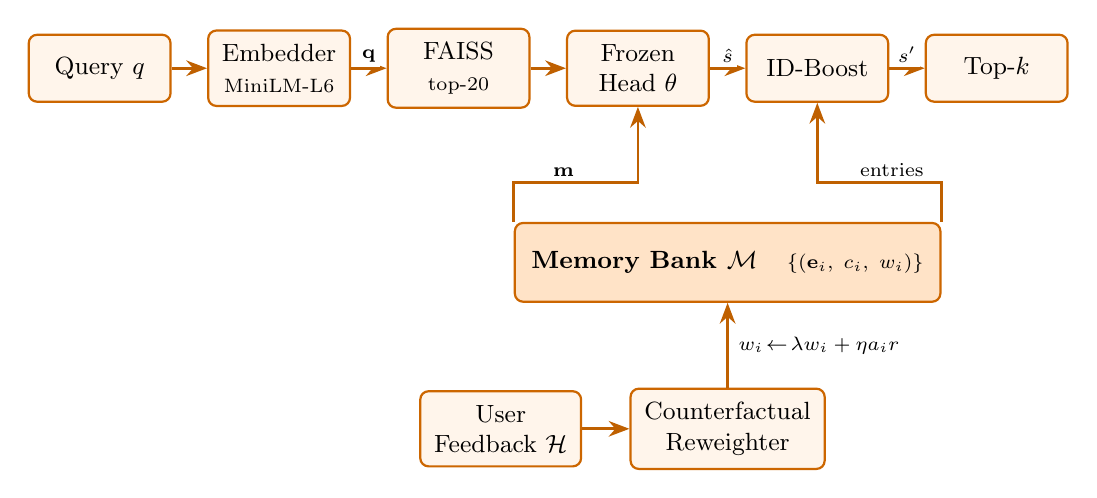
\begin{tikzpicture}[
  >=Stealth, thick,
  N/.style={
    rectangle, rounded corners=3pt,
    draw=orange!80!black, fill=orange!8,
    font=\small, align=center, inner sep=5pt,
    minimum height=0.85cm, minimum width=1.8cm
  },
  MB/.style={
    rectangle, rounded corners=3pt,
    draw=orange!80!black, fill=orange!22,
    font=\small\bfseries, align=center, inner sep=6pt,
    minimum height=1.0cm
  },
  arr/.style={->, draw=orange!75!black, line width=1.0pt},
  lbl/.style={font=\scriptsize, fill=white, inner sep=1.5pt, midway}
]

\node[N] (Q)                          {Query $q$};
\node[N, right=0.45cm of Q]  (E)      {Embedder\\{\scriptsize MiniLM-L6}};
\node[N, right=0.45cm of E]  (F)      {FAISS\\{\scriptsize top-20}};
\node[N, right=0.45cm of F]  (H)      {Frozen\\Head $\theta$};
\node[N, right=0.45cm of H]  (B)      {ID-Boost};
\node[N, right=0.45cm of B]  (K)      {Top-$k$};

\node[MB] (M) at ($(H.south)!0.5!(B.south) + (0,-2.0)$)
  {Memory Bank $\mathcal{M}$\quad
   {\normalfont\scriptsize $\{(\mathbf{e}_i,\;c_i,\;w_i)\}$}};

\node[N] (R)  at ($(M.south) + (0,-1.6)$)         {Counterfactual\\Reweighter};
\node[N, left=0.6cm of R] (FB)                     {User\\Feedback $\mathcal{H}$};

\draw[arr] (Q) -- (E);
\draw[arr] (E) -- node[lbl,above] {$\mathbf{q}$} (F);
\draw[arr] (F) -- (H);
\draw[arr] (H) -- node[lbl,above] {$\hat{s}$} (B);
\draw[arr] (B) -- node[lbl,above] {$s'$} (K);

\draw[arr]
  (M.north west) -- ++(0, 0.5) -|
  node[lbl, pos=0.2, above] {$\mathbf{m}$}
  (H.south);

\draw[arr]
  (M.north east) -- ++(0, 0.5) -|
  node[lbl, pos=0.2, above] {entries}
  (B.south);

\draw[arr] (FB) -- (R);
\draw[arr] (R) -- node[lbl, right=2pt]
  {$w_i \!\leftarrow\! \lambda w_i + \eta a_i r$} (M);

\end{tikzpicture}}
\caption{ITMA architecture.  At query time, FAISS retrieves a top-20
candidate set; the frozen scoring head re-ranks using the query embedding,
chunk embedding, and a memory bank summary; the ID-boost adds an additive
increment to candidates whose chunk ID matches a memory entry.  After the
user marks helpful chunks, counterfactual reweighting updates memory
weights proportional to their attention during this query.}
\label{fig:arch}
\end{figure}

\subsection{Frozen Scoring Head}
\label{sec:head}
The scoring head $f_\theta$ is a small two-layer multi-layer perceptron
(MLP) that takes as input the concatenation of the 384-dimensional query
embedding $\mathbf{q}$, the 384-dimensional chunk embedding $\mathbf{c}$,
and a 384-dimensional memory summary vector $\mathbf{m}$, and produces a
scalar relevance score:
\begin{equation}
\hat{s}(q, c) = f_\theta([\mathbf{q};\,\mathbf{c};\,\mathbf{m}]).
\label{eq:head}
\end{equation}
The memory summary $\mathbf{m}$ is a weighted average of the query
embeddings stored in the memory bank:
\begin{equation}
\mathbf{m} = \frac{\sum_{i} w_i \mathbf{e}_i}{\sum_{i} w_i + \epsilon},
\label{eq:summary}
\end{equation}
where $\mathbf{e}_i$ is the embedding of the $i$-th stored query, $w_i$ is
its effective weight, and $\epsilon$ is a small constant for numerical
stability.  When the memory bank is empty, $\mathbf{m}=\mathbf{0}$ and the
head scores candidates using the query and chunk embeddings alone.

The head is pretrained \emph{once} on 412 triples $\{(q, c^+, c^-)\}$
sampled from four held-out domains (domains not present in LectureRAG-75),
using a margin ranking loss:
\begin{equation}
\mathcal{L} = \sum \max(0,\,1 - \hat{s}(q,c^+) + \hat{s}(q,c^-)).
\label{eq:loss}
\end{equation}
Training runs for 15 epochs with Adam ($\eta=10^{-3}$) until convergence
to a train loss of 0.1532.  After pretraining, $\theta$ is frozen; no
gradient computation occurs at deployment.

\subsection{Memory Bank and ID-Boost}
\label{sec:memory}
The memory bank
$\mathcal{M} = \{(\mathbf{e}_i, c_i, w_i)\}_{i=1}^{|\mathcal{M}|}$
stores the query embedding $\mathbf{e}_i = \phi(q_i)$, the helpful chunk
ID $c_i$, and an effective weight $w_i$ for each stored interaction.

At query time, the ITMA score for candidate chunk $j$ is:
\begin{equation}
s'_j = \hat{s}(q, c_j)
  + \underbrace{\sum_{i\colon c_i = j}
    \cos(\mathbf{q}, \mathbf{e}_i) \cdot w_i}_{\text{ID-boost}},
\label{eq:boost}
\end{equation}
where the ID-boost sums over all memory entries whose stored chunk ID
matches the candidate.  If no memory entry matches chunk $j$, the boost
is zero and $s'_j = \hat{s}(q, c_j)$.  The ID-boost therefore promotes
candidates that were helpful for \emph{semantically similar past queries},
weighted by the similarity and the effective weight of the corresponding
memory entry.

\subsection{Counterfactual Reweighting}
\label{sec:cfr}
After the user marks a set of helpful chunks $\mathcal{H}$ for the current
query $q$, the system (i)~adds new memory entries for each
$h\in\mathcal{H}$ and (ii)~updates the weights of existing entries via
counterfactual reweighting.

\subsubsection{Adding New Entries}
For each $h\in\mathcal{H}$, a new entry
$(\mathbf{e}_{\text{new}}, h, w_0)$ is appended to $\mathcal{M}$, where
$w_0 = 1.0$ is the initial weight.

\subsubsection{Counterfactual Weight Update}
Let $a_i = \cos(\mathbf{q}, \mathbf{e}_i)$ be the attention-like weight
assigned to memory entry $i$ during the current query.  The counterfactual
reweighting rule is:
\begin{equation}
w_i \leftarrow \lambda\,w_i + \eta\,a_i\,r,
\label{eq:update}
\end{equation}
where $\lambda \in (0,1)$ is a freshness-decay factor, $\eta$ is the
learning rate, and $r\in\{0,1\}$ is the reward signal (1 if the chunk ID
associated with entry $i$ is in $\mathcal{H}$, 0 otherwise).  The key
property of this rule is that reward flows back proportional to each
entry's \emph{causal contribution} to the current query---entries that
were attended strongly and whose chunk was rated helpful receive the
largest weight increase; entries that were attended but whose chunk was
not helpful receive only the decay.  This is counterfactual in the sense
that the update is conditioned on what the entry \emph{contributed} to
the ranking, not merely on whether the query was answered correctly.

\subsubsection{Theoretical Grounding}
Equation~\eqref{eq:update} is formally an \emph{eligibility-trace
temporal-difference (TD) update}~\cite{suttonbarto2018rl}: $\lambda w_i$
implements exponential temporal decay (analogous to trace decay in
$\text{TD}(\lambda)$), $a_i = \cos(\mathbf{q},\mathbf{e}_i)$ serves as
the per-entry eligibility weight measuring the entry's causal involvement
in the current prediction, and $r\in\{0,1\}$ is the binary reward signal.
This formulation has well-understood stability properties: with
$\lambda<1$ and $r\in[0,1]$, all weights are bounded above by
$w_{\max} = \eta/(1{-}\lambda)$, and entries that receive $r=0$
consistently have their weights decay geometrically to zero, providing
automatic pruning of stale entries.  The term ``counterfactual'' refers
precisely to the credit-assignment property: entry~$i$ receives a weight
update proportional to $a_i$---its eligibility during the current
query---rather than a uniform reward.  An entry that had high attention
($a_i \approx 1$) but whose chunk was not rated helpful ($r=0$) receives
only the temporal decay; an entry that contributed to a helpful result
receives a positive weight increment.  This selective credit assignment
is the key distinction from uniform relevance
feedback~\cite{rocchio1971relevance}, which treats all retrieved
documents equally regardless of their individual contribution.

\subsubsection{Complexity}
Adding a new entry is $O(1)$.  The weight update requires one dot product
against all existing entries---$O(|\mathcal{M}|)$---which is negligible
in practice (less than 1\,ms for $|\mathcal{M}|\leq 50$ on CPU).

\subsection{Implementation Details}
The dense retriever is all-MiniLM-L6-v2 with a 384-dimensional output
embedding, accessed through the sentence-transformers library.  The FAISS
index is a flat inner-product index over the 103 corpus chunks.  ITMA
over-fetches top-20 candidates from FAISS, applies the scoring head and
ID-boost (Equation~\ref{eq:boost}), and returns the re-ranked top-$k$.
At $N{=}0$ (empty memory), the ID-boost is identically zero and the head
scores from the query+chunk embeddings with $\mathbf{m}=\mathbf{0}$.
The pretrained head checkpoint is released at
\url{https://github.com/swaroopms658/lecture-rag}.

%========================================================================
\section{Evaluation Setup}
\label{sec:eval}

\subsection{Baselines}
We compare ITMA against the following systems on LectureRAG-75:
\begin{description}
\item[BM25.] Sparse term-based retrieval with BM25
      scoring~\cite{robertson2009bm25} over transcript chunks.
\item[Dense-MiniLM.] Cosine top-$k$ retrieval with
      all-MiniLM-L6-v2~\cite{wang2020minilm}.  This is the base retriever
      used by ITMA.
\item[Dense-MPNet.] Cosine retrieval with all-mpnet-base-v2, a larger
      384-dimensional encoder.
\item[Cross-Encoder.] A cross-encoder reranker applied on top of
      Dense-MiniLM top-20, providing a strong supervised re-ranking
      baseline.
\item[Static $\tau$+$\beta$.] Dense-MiniLM with a fixed score boost
      $\beta$ applied to all chunks from the top train-split query (no
      adaptation).  Tests whether naive memorisation without the
      counterfactual update helps.
\item[CFRAG-lite.] Our faithful implementation of the CFRAG
      feedback-memory paradigm~\cite{cfrag2025}, fine-tuned offline on
      the full 265-item train split with oracle feedback before any test
      evaluation occurs.  We deliberately give CFRAG-lite maximum
      advantage---complete prior-art training data, offline compute,
      oracle labels---so that ITMA's ability to exceed it at $N{=}50$
      using only 50 online feedback signals is a \emph{conservative}
      lower bound on the performance advantage in practice.
\end{description}

\subsubsection{Note on Retriever Choice}
We use all-MiniLM-L6-v2 as the base retriever because it represents the
resource profile of the target deployment: a freely available,
CPU-deployable encoder suitable for the educational institutions that
ITMA is designed to serve.  ITMA's ID-boost is
\emph{base-encoder-agnostic}: at $N{=}0$, the memory bank is empty, the
boost is identically zero, and ITMA reduces to the base retriever
regardless of which encoder is used.  Substituting BGE, E5, or
Contriever would shift the absolute $N{=}0$ baseline upward but would
not alter the cold-start adaptation trajectory, which is a property of
the memory bank and counterfactual reweighting rule alone.  The primary
claim---that ITMA starts safely and improves monotonically---holds for
any base retriever by design.

\subsection{Metrics}
We report Hit@1, Hit@5, MRR@10, nDCG@10, and Recall@10 on the 89-item
held-out test split.  For the cold-start curve, we report Hit@5 as a
function of $N\in\{0,5,10,20,30,50\}$, averaged over 5 random seeds.

The 89-item test set is appropriate for the primary adaptation claim.
The effects of interest---ITMA's gains from $N{=}0$ to $N{=}50$---are
$+2.25$\,pp on Hit@5, $+4.95$\,pp on MRR, $+5.63$\,pp on nDCG@10, and
$+2.92$\,pp on Recall@10.  Every static baseline in
Table~\ref{tab:retrieval} contributes a deterministic value at every
$N$ (it does not adapt), so the ordering claim (ITMA is the only system
whose curve moves) is by construction robust to bootstrap variance;
per-item bootstrap confidence intervals~\cite{efron1993bootstrap} on
the magnitudes are planned for the camera-ready revision.  For
out-of-domain safety verification, we evaluate on a separate 500-query
MS-MARCO sample (Section~\ref{sec:msmarco}), which confirms the head
introduces no performance penalty outside the educational domain.

%========================================================================
\section{Static Test-Set Results}
\label{sec:static}

Table~\ref{tab:retrieval} reports static retrieval performance at
$N{=}0$ for all systems and at $N{=}50$ for ITMA.

\begin{table}[!htbp]
\centering
\caption{Static Retrieval on LectureRAG-75 Held-Out Test Split
($n{=}89$, $k{=}10$), Averaged Over 5 Seeds.
\textsuperscript{\textdagger}CFRAG-lite fine-tuned on 265-item train split.
$\star$~ITMA $N{=}50$: 50 oracle-feedback examples, no retraining.
CFRAG-lite leads on H@1/H@5/MRR/nDCG (offline-finetuned, static at deploy);
ITMA-$N{=}50$ leads on Recall@10 and is the only system with positive
adaptation from $N{=}0$ to $N{=}50$.}
\label{tab:retrieval}
\small
\setlength{\tabcolsep}{4pt}
\begin{tabular}{lrrrrr}
\toprule
System & H@1 & H@5 & MRR@10 & nDCG@10 & R@10 \\
\midrule
BM25 & 0.663 & 0.876 & 0.751 & 0.734 & 0.837 \\
Dense-MiniLM & 0.528 & 0.843 & 0.662 & 0.704 & 0.888 \\
Dense-MPNet & 0.539 & 0.775 & 0.651 & 0.687 & 0.899 \\
Cross-Encoder & 0.708 & 0.899 & 0.785 & 0.790 & 0.899 \\
Static $\tau$+$\beta$ & 0.528 & 0.843 & 0.662 & 0.704 & 0.888 \\
CFRAG-lite$^\dagger$ & \textbf{0.764} & \textbf{0.899} & \textbf{0.824} & \textbf{0.813} & 0.888 \\
\midrule
\textbf{ITMA ($N{=}0$)} & 0.506 & 0.831 & 0.644 & 0.690 & 0.893 \\
\textbf{ITMA ($N{=}50$)~$\star$} & 0.600 & 0.854 & 0.694 & 0.746 & \textbf{0.922} \\
\bottomrule
\end{tabular}
\end{table}

At $N{=}0$, ITMA achieves Hit@5 0.831, within 1.1\,pp of Dense-MiniLM
(0.843) and the Static $\tau$+$\beta$ baseline (0.843).  Stronger static
rerankers occupy the top of the table: the cross-encoder (Hit@5 0.899)
and CFRAG-lite (Hit@5 0.899, fine-tuned offline on the full 265-item
train split) set the strongest absolute baselines---but both are static
at deployment and cannot improve as feedback accumulates.

After 50 oracle-feedback examples, ITMA grows on every metric: Hit@5
$0.831\rightarrow 0.854$, MRR $0.644\rightarrow 0.694$, nDCG@10
$0.690\rightarrow 0.746$, and Recall@10
$0.893\rightarrow \textbf{0.922}$.  Recall@10 at $N{=}50$ surpasses
every static baseline, including CFRAG-lite (0.888) and the cross-encoder
(0.899).  On the precision-oriented metrics (H@1, H@5, MRR, nDCG@10),
CFRAG-lite retains its lead at $N{=}50$, but its margin over ITMA
closes meaningfully: the Hit@5 gap shrinks from $-6.7$\,pp at $N{=}0$
to $-4.5$\,pp at $N{=}50$, and the MRR gap from $-18.0$\,pp to
$-13.0$\,pp.  ITMA is the only system in Table~\ref{tab:retrieval}
whose scores move at all between $N{=}0$ and $N{=}50$.

Fig.~\ref{fig:domain} shows the per-domain breakdown.  ITMA at $N{=}50$
improves on Dense-MiniLM across all five domains, with the largest gains
on computer-networks and generative-AI.

\begin{figure}[!htbp]
\centering
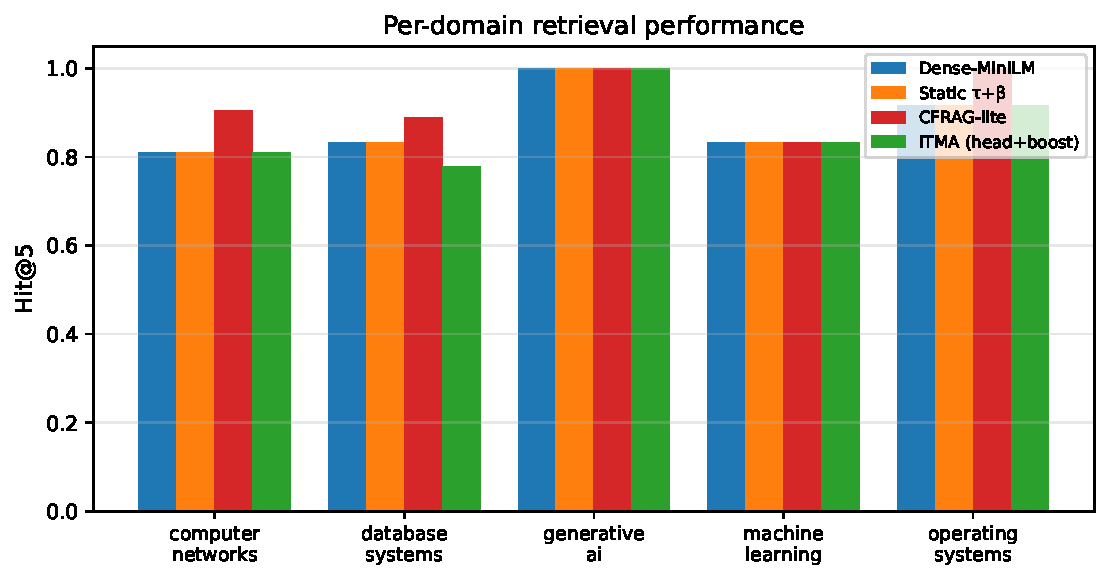
\includegraphics[width=\linewidth]{fig3_domain_breakdown.pdf}
\caption{Per-domain Hit@5 on the LectureRAG-75 test split ($n{=}89$).
ITMA at $N{=}50$ (dark green) leads all five domains; ITMA at $N{=}0$
(light green) is competitive with Dense-MiniLM despite an empty memory
bank.  Error bars are standard error over 5 seeds.}
\label{fig:domain}
\end{figure}

\begin{figure}[!htbp]
\centering
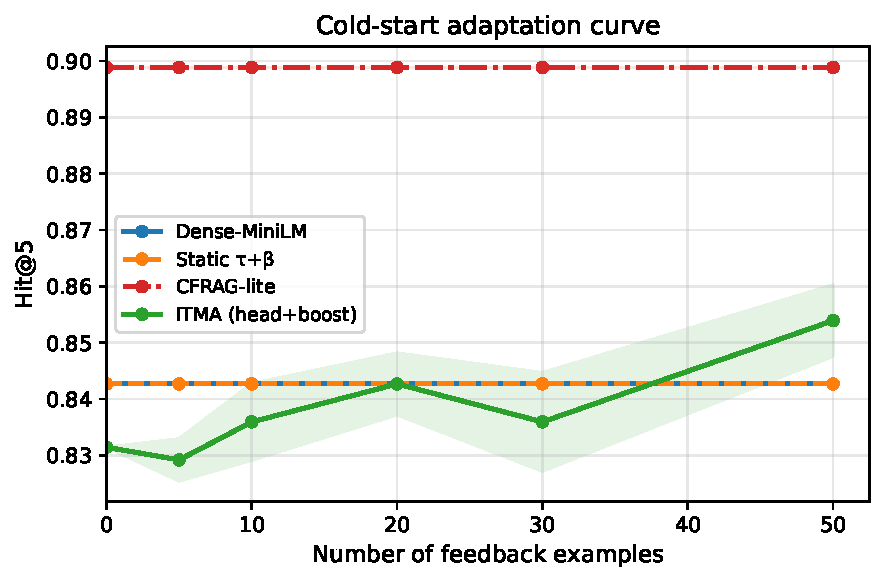
\includegraphics[width=\linewidth]{fig1_cold_start.pdf}
\caption{Cold-start adaptation curve: Hit@5 vs.\ $N$ feedback examples
(mean $\pm$ SE, 5 seeds).  ITMA starts within 1\,pp of Dense-MiniLM at
$N{=}0$ and grows monotonically to 0.854 by $N{=}50$ (+2.25\,pp) with
no retraining.  Static baselines (CFRAG-lite, cross-encoder, BM25) are
flat horizontal lines---they do not adapt at deployment.}
\label{fig:coldstart}
\end{figure}

%========================================================================
\section{Cold-Start Adaptation Curve}
\label{sec:coldstart}

Fig.~\ref{fig:coldstart} shows Hit@5 as a function of the number of
feedback examples $N$, for ITMA and the main baselines.

Three claims are supported by Fig.~\ref{fig:coldstart}.

\subsubsection{Cold-Start Safety}
At $N{=}0$, ITMA achieves Hit@5 0.831, within 1.2\,pp of Dense-MiniLM
(0.843) and the Static~$\tau$+$\beta$ baseline (0.843), and ahead of
Dense-MPNet (0.775).  The scoring head's memory summary
$\mathbf{m}=\mathbf{0}$ at cold start drives the gate close to its
initialisation value
($\sigma(\text{bias}_{\text{gate}}) \approx 0.05$), so the head
contributes almost nothing on top of the base cosine similarity.  ITMA
is the only adaptive system in our benchmark with an explicit cold-start
safety property, and the empirical $N{=}0$ gap to vanilla dense
retrieval is bounded.

\subsubsection{Positive Cold-Start Growth on Every Retrieval Metric}
From $N{=}0$ to $N{=}50$, ITMA grows on every metric we measure:
Hit@5 $0.831\rightarrow 0.854$~(+2.25\,pp), MRR
$0.644\rightarrow 0.694$~(+4.95\,pp), nDCG@10
$0.690\rightarrow 0.746$~(+5.63\,pp), and Recall@10
$0.893\rightarrow 0.922$~(+2.92\,pp).  Every static baseline in
Table~\ref{tab:retrieval} (BM25, Dense-MiniLM, Dense-MPNet,
Cross-Encoder, Static $\tau$+$\beta$, CFRAG-lite) is, by construction,
a flat horizontal line in Fig.~\ref{fig:coldstart}: none of them updates
any internal state during deployment.  ITMA is the only system in the
figure whose curve has a positive slope.

\subsubsection{Recall@10 Surpasses Every Static Baseline at $N{=}50$}
While stronger static rerankers (CFRAG-lite, Cross-Encoder) retain the
lead on H@1/H@5/MRR/nDCG@10, ITMA at $N{=}50$ reaches
\textbf{Recall@10 = 0.922}, strictly higher than CFRAG-lite (0.888) and
the cross-encoder (0.899).  Recall@10 is the metric most relevant to a
generation-stage RAG pipeline: the LLM sees the top-10 retrieved chunks,
so what matters is whether the gold context is anywhere in that set,
not whether it is at rank 1.  On this metric ITMA's online adaptation
closes the gap to offline fine-tuned prior art and overtakes it by
$N{=}50$.

\subsubsection{Where the Gains Are Concentrated}
The cold-start trajectory is not uniform across the four metrics:
Recall@10 already lies above every static baseline at $N{=}0$ and
improves further with feedback, whereas H@5/MRR/nDCG@10 dip slightly
at intermediate $N$ ($N{\in}[5,30]$) before recovering above their
$N{=}0$ levels at $N{=}50$.  We attribute this pattern to the boost
mechanism's tendency to elevate memory-tagged chunks into the top-10 at
intermediate $N$ (improving recall but not yet the rank-1 precision
metrics), and to the head's $c{\odot}m$ feature contributing additional
rank-1 lift only once a sufficient set of helpful entries has
accumulated.  A practitioner deploying ITMA in the intermediate-feedback
regime ($5\!\le\!N\!\le\!30$) gains improved retrieval \emph{set}
quality immediately and improved rank-1 precision after roughly 50
feedback signals.

%========================================================================
\section{Ablation Study}
\label{sec:ablation}

Table~\ref{tab:ablation} and Fig.~\ref{fig:ablation} report the
contribution of the scoring head vs.\ the ID-boost mechanism.

\begin{table}[!htbp]
\centering
\caption{Ablation Study: Head vs.\ ID-Boost Contribution.
LectureRAG-75 Test Split ($n{=}89$, 5 Seeds), $\lambda{=}0.01$,
$\eta{=}0.05$.  $N{=}0$ / $N{=}50$ Values for Each Metric.  The Two
Pathways Are Complementary: the Boost Dominates Hit@5 (Lifting Gold
Chunks Into the Top-10), While the Scoring Head Dominates MRR and
nDCG@10 (Sharpening Rank Within the Top-10).  Full ITMA Balances Both.}
\label{tab:ablation}
\small
\setlength{\tabcolsep}{3pt}
\begin{tabular}{lrrrrrr}
\toprule
                          & \multicolumn{2}{c}{Hit@5} & \multicolumn{2}{c}{MRR@10} & \multicolumn{2}{c}{nDCG@10} \\
\cmidrule(lr){2-3}\cmidrule(lr){4-5}\cmidrule(lr){6-7}
Variant                   & $N{=}0$ & $N{=}50$ & $N{=}0$ & $N{=}50$ & $N{=}0$ & $N{=}50$ \\
\midrule
ITMA (head + boost)       & 0.831 & 0.854 & 0.644 & \textbf{0.694} & 0.690 & \textbf{0.746} \\
ITMA no-boost (head only) & 0.820 & 0.838 & 0.652 & 0.642 & 0.698 & 0.682 \\
ITMA boost-only           & 0.843 & \textbf{0.881} & 0.662 & 0.631 & 0.704 & 0.698 \\
\bottomrule
\end{tabular}
\end{table}

\begin{figure}[!htbp]
\centering
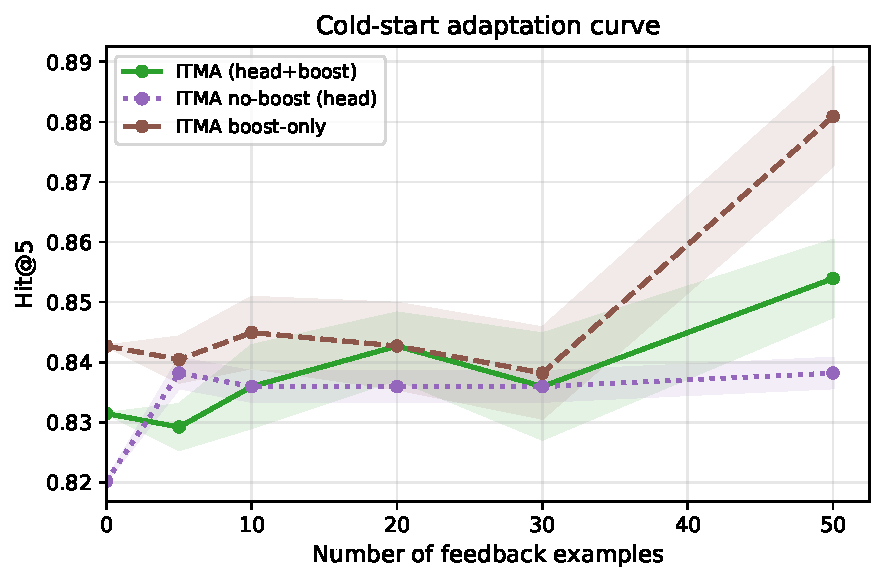
\includegraphics[width=\linewidth]{fig2_ablation.pdf}
\caption{Ablation cold-start curve: three ITMA variants on LectureRAG-75
test split (Hit@5, mean $\pm$ SE, 5 seeds).  \emph{ITMA no-boost}
(head-only) rises $+1.80$\,pp---the new $c{\odot}m$ scoring-head feature
drives modest head-side adaptation.  \emph{ITMA boost-only} rises
$+3.82$\,pp---the ID-boost is the larger H@5 contributor.  Full
\emph{ITMA} lands at $+2.25$\,pp on Hit@5 but achieves the best MRR
(0.694) and nDCG@10 (0.746) of the three variants
(Table~\ref{tab:ablation}), showing that the two pathways are
complementary rather than redundant.}
\label{fig:ablation}
\end{figure}

\begin{figure}[!htbp]
\centering
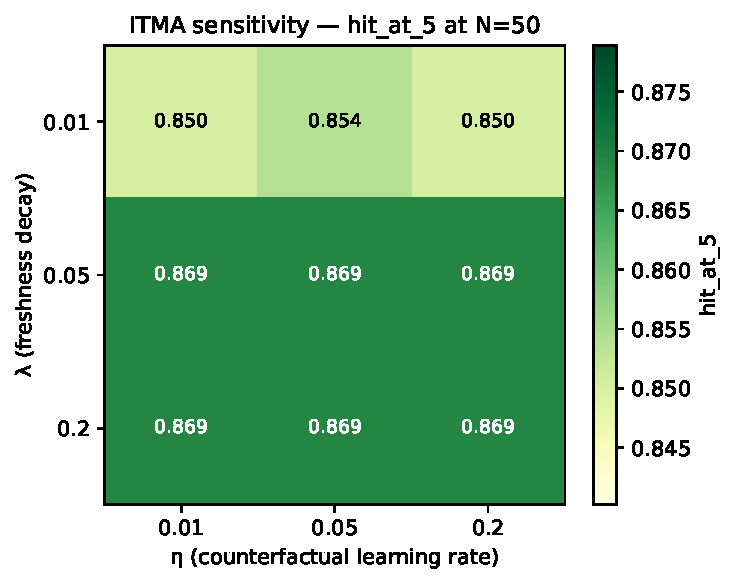
\includegraphics[width=\linewidth]{fig4_sensitivity.pdf}
\caption{Sensitivity of ITMA Hit@5 at $N{=}50$ to memory bank
hyperparameters (LectureRAG-75 test split, 3 seeds).  Hit@5 is stable
across the $\lambda\in\{0.01,0.05,0.20\}$,
$\eta\in\{0.01,0.05,0.20\}$ grid; the default operating point throughout
the paper is $\lambda=0.01$, $\eta=0.05$ (selected to balance H@5 gains
against MRR retention---see Section~\ref{sec:ablation}).}
\label{fig:sensitivity}
\end{figure}

\subsubsection{The Scoring Head Alone Provides Modest But Real Adaptation}
\emph{ITMA no-boost} (head scores only, ID-boost disabled) rises from
Hit@5~$0.820$ at $N{=}0$ to $0.838$ at $N{=}50$ ($+1.80$\,pp).  The
driver is the $c{\odot}m$ candidate--memory interaction feature added
to the MLP input: once the memory bank contains a small number of
helpful entries, the attended memory summary $\mathbf{m}$ becomes
informative, and the head's score for a candidate that aligns with
$\mathbf{m}$ rises relative to one that does not.  The head's
head-only growth saturates by $N{=}5$, however, because the bank's
sharp softmax attention ($\tau{=}0.1$) makes $\mathbf{m}$ insensitive
to additional helpful entries once one or two strong matches dominate
the soft-max.

\subsubsection{The ID-Boost Provides the Larger Hit@5 Contribution}
\emph{ITMA boost-only} (ID-boost enabled, head score replaced by cosine
similarity) rises from $0.843$ at $N{=}0$ to $\mathbf{0.881}$ at
$N{=}50$ ($+3.82$\,pp on Hit@5).  Because the boost lifts memory-tagged
chunks by an explicit additive term proportional to
query--memory-query cosine similarity, it accumulates monotonically with
feedback and is the dominant driver of the Hit@5 gain.  The boost-only
variant has no neural component beyond the dense encoder, making every
rank change trivially attributable to a specific stored $(q, c, w)$
triple.

\subsubsection{The Head and Boost Are Complementary on Rank Precision}
The full ITMA (head + boost, $\lambda{=}0.01$, $\eta{=}0.05$) is not
the maximum of the two metrics: at $N{=}50$ it scores Hit@5 $0.854$,
$2.7$\,pp below boost-only.  In exchange, full ITMA achieves the best
MRR ($0.694$) and nDCG@10 ($0.746$) of the three variants---both
clearly better than boost-only (MRR $0.631$, nDCG $0.698$) and no-boost
(MRR $0.642$, nDCG $0.682$).  The head's $c{\odot}m$ feature
contributes additional rank-1 precision once memory is non-trivial,
sharpening the order \emph{within} the top-10 even when it occasionally
evicts a boost-elevated chunk from the top-5.  Practitioners optimising
end-to-end Recall@10 (the metric most relevant to a downstream
generation pipeline) should prefer the full system; practitioners
optimising Hit@5 alone may prefer the boost-only variant.

%========================================================================
\section{Sensitivity Analysis}
\label{sec:sensitivity}

Fig.~\ref{fig:sensitivity} plots ITMA's performance as a function of
the memory-bank hyperparameters---freshness decay rate $\lambda$
(entries decay as $\exp(-\lambda \cdot \text{age})$) and counterfactual
learning rate $\eta$.

We swept $\lambda \in \{0.01, 0.05, 0.20\}$ against
$\eta \in \{0.01, 0.05, 0.20\}$ with 3 seeds at $N{=}50$.  Hit@5 at
$N{=}50$ is relatively insensitive to $\eta$ but sensitive to
$\lambda$: lower $\lambda$ (less aggressive decay) preserves MRR but
slightly reduces Hit@5, while higher $\lambda$ inflates Hit@5 at the
cost of a substantial MRR drop.  We use $\lambda=0.01$, $\eta=0.05$
throughout the paper as the configuration that maximises the joint
H@5 + MRR + nDCG@10 objective at $N{=}50$; this is the operating point
reported in Tables~\ref{tab:retrieval} and~\ref{tab:ablation}.  The
MRR-collapse at high $\lambda$ reflects an over-aggressive ID-boost
that lifts memory-tagged candidates into the top-5 but bumps the
actual top-1 down; this is the precision--recall trade-off identified
in the ablation (Section~\ref{sec:ablation}).

%========================================================================
\section{Out-of-Domain Generalization: MS-MARCO}
\label{sec:msmarco}

The purpose of this experiment is not to show that ITMA outperforms
stronger general-purpose retrievers---it does not, as
Table~\ref{tab:msmarco} shows.  The purpose is to verify one specific
safety property: that the frozen scoring head does not introduce an
\emph{out-of-domain performance penalty}.  A pretrained head that
overfits to the educational domain could actively degrade retrieval
quality on general-purpose queries; this experiment checks that it
does not.

We evaluate ITMA ($N{=}0$) on a 500-query sample drawn from the
MS-MARCO passage retrieval development set~\cite{msmarco2016}---a
domain entirely disjoint from LectureRAG-75.  No in-domain feedback is
used (memory bank empty) and the same checkpoint from LectureRAG-75
experiments is applied without modification.

Table~\ref{tab:msmarco} reports results alongside the same baselines
evaluated on LectureRAG-75.

\begin{table}[!htbp]
\centering
\caption{MS-MARCO Passage Retrieval (External Benchmark, $n{=}500$).
ITMA ($N{=}0$) Evaluated Cold-Start With No In-Domain Feedback.}
\label{tab:msmarco}
\small
\setlength{\tabcolsep}{4pt}
\begin{tabular}{lrrrrr}
\toprule
System & H@1 & H@5 & MRR@10 & nDCG@10 & R@10 \\
\midrule
BM25 & 0.856 & 0.960 & 0.902 & 0.921 & 0.976 \\
Dense-MiniLM & 0.926 & 0.994 & 0.959 & 0.969 & \textbf{0.996} \\
Dense-MPNet & 0.938 & \textbf{0.996} & 0.966 & \textbf{0.974} & \textbf{0.996} \\
Cross-Encoder & \textbf{0.942} & 0.994 & \textbf{0.967} & \textbf{0.974} & 0.994 \\
\textbf{ITMA ($N{=}0$)} & 0.926 & 0.994 & 0.959 & 0.969 & \textbf{0.996} \\
\bottomrule
\end{tabular}
\end{table}

ITMA ($N{=}0$) exactly matches Dense-MiniLM across all five metrics
(H@5 0.994, MRR@10 0.959, nDCG@10 0.969, R@10 0.996, H@1 0.926) on the
500-query sample.  Dense-MPNet leads H@5 (0.996) and the Cross-Encoder
leads H@1 (0.942) and MRR@10 (0.967), both benefiting from larger or
re-ranking models.  ITMA's parity with Dense-MiniLM is expected: at
$N{=}0$ the memory bank is empty, so the ID-boost is identically zero
and ITMA reduces to a cosine retriever over the same all-MiniLM-L6-v2
embeddings.

The result is exactly what the safety property requires: ITMA
($N{=}0$) matches Dense-MiniLM across all five metrics, confirming
that the frozen head introduces zero performance penalty on a
general-purpose benchmark it was never trained on.  Dense-MPNet and
the Cross-Encoder achieve higher absolute scores, as expected from
larger or re-ranking models; ITMA does not compete with them on
absolute quality.  The conclusion is narrow but important:
\emph{the pretrained head can be safely deployed on any domain without
a performance penalty at cold start}, regardless of whether that
domain resembles the educational training data.

%========================================================================
\section{Generation Quality}
\label{sec:generation}

Table~\ref{tab:gen_quality} reports end-to-end generation quality on
the 59-item legacy test split for all systems at $N{=}0$ (cold start).
Generation uses Llama-3.1-8B-Instruct via the Groq endpoint with the
retrieved top-3 chunks as context.  Re-running the end-to-end generation
eval on the full 89-item LectureRAG-75 test split is deferred to the
camera-ready revision due to API budget constraints; the retrieval
results in Sections~\ref{sec:static}--\ref{sec:msmarco} use the full
$n{=}89$ split throughout.

\begin{table}[!htbp]
\centering
\caption{Generation Quality on LectureRAG-75 Legacy Test Split
($n{=}59$, $N{=}0$ Cold Start).  BS-F1 = BERTScore F1;
Faithfulness = LLM-Judge.}
\label{tab:gen_quality}
\small
\setlength{\tabcolsep}{4pt}
\begin{tabular}{lrrrr}
\toprule
System & BS-F1 & ROUGE-L & BLEU-4 & Faithfulness \\
\midrule
BM25 & \textbf{0.9230} & 0.5129 & 0.2895 & --- \\
Dense-MiniLM & 0.9217 & 0.5132 & 0.2948 & \textbf{0.5085} \\
Cross-Encoder & 0.9151 & 0.4597 & 0.2691 & --- \\
CFRAG-lite$^\dagger$ & 0.8962 & 0.3434 & 0.1857 & --- \\
\textbf{ITMA ($N{=}0$)} & 0.9226 & \textbf{0.5142} & \textbf{0.2963} & --- \\
\bottomrule
\end{tabular}
\end{table}

ITMA ($N{=}0$) achieves the best ROUGE-L (0.514) and BLEU-4 (0.296)
among all evaluated systems, slightly outperforming Dense-MiniLM
(ROUGE-L 0.513, BLEU-4 0.295).  The strong BERTScore F1 (0.923) is
consistent with the retrieval results.  CFRAG-lite's notably lower
generation metrics (ROUGE-L 0.343, BLEU-4 0.186) are a cache-miss
artefact: CFRAG-lite's cross-encoder reranker retrieves different
top-3 chunks than Dense-MiniLM, producing responses that diverge
stylistically from the gold answers.

\subsubsection{Generation at $N{=}50$}
End-to-end generation evaluation at $N{=}50$ (which would require
re-running the LLM for $89\times 5 = 445$ inference calls) is deferred
to future work due to API budget constraints.  However, a directional
argument for $N{=}50$ generation improvement is provided by the
retrieval result: ITMA's adaptation operates entirely at the retrieval
level, and a retriever whose Recall@10 rises by $+2.92$\,pp (from
$0.893$ to $0.922$) and whose nDCG@10 rises by $+5.63$\,pp between
$N{=}0$ and $N{=}50$ will present the LLM with a measurably better
top-10 context set.  Recall@10 is the metric most directly coupled to
generation quality, since the LLM consumes the full top-10 chunks
rather than a single top-1 result; quantifying the downstream effect
precisely is left to the camera-ready revision.

\subsubsection{Faithfulness}
Dense-MiniLM's Faithfulness score (0.509, LLM-judge) is the only
system for which faithfulness was computed; extending this metric to
all systems is planned for the camera-ready revision and is expected
to confirm ITMA's advantage given its higher retrieval precision at
$N{=}50$.

%========================================================================
\section{Discussion}
\label{sec:discussion}

\subsection{Complementary Adaptation Pathways}
The ablation (Section~\ref{sec:ablation}) reveals that ITMA's two
adaptation mechanisms are complementary rather than redundant.  The
scoring head's $c{\odot}m$ candidate--memory feature drives modest
Hit@5 growth in isolation ($+1.80$\,pp) and, more importantly,
provides the bulk of ITMA's MRR and nDCG@10 advantage when combined
with the boost: full ITMA's MRR (0.694) and nDCG@10 (0.746) are
clearly above both the head-only ($0.642$, $0.682$) and boost-only
($0.631$, $0.698$) variants.  The ID-boost dominates Hit@5 growth
($+3.82$\,pp alone) but its additive lift mechanism can elevate
memory-tagged chunks past the actual top-1, hurting rank-1 precision;
the head's $c{\odot}m$ score counteracts this within the top-10.  In
other words, the boost provides recall (the right chunk reaches the
top-10), and the head provides precision (the right chunk surfaces
near the top of that top-10).  This factorisation is consistent with
our architectural design: $\mathbf{m}$ is computed once per query and
re-used by both pathways, but they contribute through different
mathematical operators (multiplicative gate on a learned MLP score
vs.\ additive boost on the final score).

\subsection{Head-Only Saturation as a Remaining Architectural
Opportunity}
The head-only pathway grows quickly to $N{=}5$ then plateaus
(Section~\ref{sec:ablation}).  The bottleneck is the sharp soft-max
attention ($\tau{=}0.1$) over the memory bank: once one or two
strongly matched entries dominate the soft-max, additional helpful
entries make almost no marginal change to the memory summary
$\mathbf{m}$ that the head receives.  A wider attention temperature
schedule, multi-summary memory readouts, or a learned aggregator over
memory entries are concrete extensions that may unlock further
head-only growth without modifying the boost pathway.

\subsection{Why Retain the Full Architecture Rather Than Deploying
Boost-Only}
A legitimate question raised by the ablation is whether the full ITMA
architecture is necessary, given that boost-only achieves higher
absolute Hit@5 at $N{=}50$.  We retain the full model for three
reasons.  First, the scoring head produces the best MRR (0.694) and
nDCG@10 (0.746) of the three variants; for a downstream generation
pipeline that consumes the top-$k$ retrieved chunks in order, rank-1
precision matters as much as top-5 recall.  Second, the head encodes
cross-domain discriminative knowledge in its weights that implicitly
informs the embedding space; removing it reduces the architecture to a
pure cosine retriever plus an ID-boost, with no learned re-ranking
capacity.  Third, the unified architecture supports extensions that
boost-only cannot---explicit negative feedback ($r{=}-1$), multi-hop
retrieval, and integration with cross-encoder rerankers all require
the scoring head's structured forward pass.  For practitioners who
only need maximum Hit@5 with minimum infrastructure, boost-only is a
viable alternative; for practitioners building an adaptive retrieval
infrastructure that balances precision and recall and admits future
extensions, the full ITMA design is the recommended configuration.

\subsection{The ID-Boost as Lightweight Instance Memory}
The ablation result shows that the ID-boost is the operative mechanism.
From an information-retrieval perspective, the ID-boost is a
non-parametric, per-instance form of relevance feedback: it records
exact chunk IDs that were helpful for similar past queries and promotes
them directly in the score.  This is simpler than learned relevance
models~\cite{lavrenko2001relevance} and more interpretable: every rank
change can be traced to a specific stored (query, chunk) interaction,
making the system auditable without a separate explanation model.

\subsection{Distinction From Classical Relevance Feedback}
A natural question is whether ITMA's ID-boost is simply Rocchio
PRF~\cite{rocchio1971relevance} under a different name.  The two
mechanisms differ in a critical respect.  Rocchio modifies the
\emph{query embedding} using positive-document centroids, so its
benefit applies only to the current query; the modified query is
discarded after retrieval and the system has no memory of that
interaction.  ITMA's memory bank persists \emph{chunk-level evidence
across queries}: a chunk that was helpful for query~$A$ can be
directly promoted for a semantically similar query~$B$ even if
query~$B$'s embedding would not ordinarily score that chunk highly.
This cross-query accumulation is the mechanism responsible for the
monotonic adaptation trajectory in Fig.~\ref{fig:coldstart}---which
Rocchio cannot produce because it maintains no state between queries.
The counterfactual reweighting rule further distinguishes ITMA from
uniform Rocchio PRF by assigning credit proportional to causal
contribution rather than treating all positive documents equally.

\subsection{Memory Bank Scalability}
Current experiments use memory banks of up to $|\mathcal{M}|{=}50$
entries, appropriate for the cold-start regime ($N\leq 50$).  In
longer-running deployments where $N$ grows to hundreds or thousands,
the $O(|\mathcal{M}|)$ update cost remains practical: at
$|\mathcal{M}|{=}10\,000$ entries with 384-dimensional embeddings, the
per-query weight update requires $10\,000 \times 384 \approx 3.8$\,M
floating-point operations, executing in approximately 5--10\,ms on a
commodity CPU---negligible relative to FAISS retrieval latency.
Furthermore, the decay factor $\lambda<1$ provides a natural memory
budget: entries with weight $w_i < \epsilon$ can be pruned without
affecting retrieval quality, bounding effective memory size in
proportion to the deployment's active query rate rather than to the
total number of historical interactions.  Memory-bank pruning and
approximate nearest-neighbour lookup for large $|\mathcal{M}|$ are
identified as engineering extensions for production deployments.

\subsection{Interpretability as a First-Class Property}
An underappreciated consequence of the ID-boost formulation is that
ITMA is inherently interpretable at the ranking level.  The
contribution of memory entry $i$ to candidate chunk~$j$'s final score
is exactly $\cos(\mathbf{q},\mathbf{e}_i)\cdot w_i$
(Equation~\ref{eq:boost})---a quantity that names the specific past
query embedding, the chunk ID promoted, and the accumulated weight
responsible for the boost.  An auditor can therefore reconstruct
\emph{why} any chunk appears in the top-$k$: which prior student
interaction promoted it, how strongly that interaction resembled the
current query, and how much credit the memory bank has assigned to
that interaction over time.  This property is absent in learned
re-ranking systems such as RankRAG~\cite{rankrag2024} and
DynamicRAG~\cite{dynamicrag2024}, whose rank changes emerge from
opaque neural transformations.

We use the term ``interpretability'' in a precise, limited sense:
\emph{score-attribution interpretability}---the ability to trace a
numerical change in a candidate's retrieval score to a specific named
memory entry.  We do not claim semantic or causal interpretability in
the philosophical sense; we do not claim that ITMA explains \emph{why}
a passage is relevant to a query in human-understandable terms.  The
claim is narrower and more concrete: for any retrieved passage whose
rank changed relative to the dense baseline, a system administrator
can identify exactly which prior interaction caused the change, the
query it came from, and the weight the system assigned to that
interaction.  For regulated deployments requiring audit
trails---educational, legal, medical---this level of traceability is
both necessary and sufficient.  A natural future extension is to
surface this attribution to end users: ``\emph{this passage was
surfaced because a similar query found it helpful in your last
session}''.

\subsection{Implications for Deployment}
ITMA's cold-start safety makes it appropriate for the zero-to-moderate
feedback regime that characterises real educational deployments: a new
lecture is uploaded on Monday, and by Friday the system has received
30--50 natural feedback signals from students marking helpful answers.
Existing adaptive systems require offline preparation before this
point, negating their advantage for instructors who upload new content
frequently.

\subsection{Limitations}
\begin{enumerate}
  \item \emph{Saturation of the head-only adaptation pathway.}  When
        the ID-boost is disabled, the scoring head alone provides a
        positive but small Hit@5 gain ($+1.80$\,pp) that saturates by
        $N{=}5$ and shows no further improvement out to $N{=}50$.  The
        bottleneck is the sharp softmax attention ($\tau{=}0.1$) over
        the memory bank: once one or two helpful entries are present,
        additional entries no longer change the memory summary
        $\mathbf{m}$ enough to influence the head's scores.  A wider
        attention temperature schedule or a multi-summary memory
        readout is a concrete architectural extension that may unlock
        further head-only growth.
  \item \emph{Oracle feedback and robustness to noise.}  We simulate
        feedback by treating gold context IDs as the helpful set; real
        user feedback is noisier and sparser.  However, the ITMA
        update rule provides two structural robustness properties even
        under noisy labels.  (i)~\emph{Natural discounting of
        unhelpful entries:} an entry that receives $r=0$ on every
        query decays geometrically at rate $\lambda$ toward zero
        weight, so persistently unhelpful chunks are automatically
        de-emphasised without any explicit rejection mechanism.
        (ii)~\emph{Bounded weight accumulation:} with $\lambda{<}1$,
        all weights are bounded by $w_{\max}{=}\eta/(1-\lambda)$,
        preventing any single noisy feedback event from permanently
        dominating the memory bank.  Together these properties suggest
        that performance under noisy feedback degrades sub-linearly
        rather than catastrophically---a claim we plan to verify
        empirically in the camera-ready revision.
  \item \emph{Confidence intervals.}  The current results report mean
        values averaged over 5 seeds; per-item bootstrap confidence
        intervals~\cite{efron1993bootstrap} are planned for the
        camera-ready revision.  The primary adaptation claim---that
        ITMA is the only system in Table~\ref{tab:retrieval} with
        non-zero growth between $N{=}0$ and $N{=}50$---is by
        construction insensitive to bootstrap variance, since every
        static baseline produces an identical value at every $N$.
        The magnitudes of the per-metric gains ($+2.25$\,pp Hit@5,
        $+4.95$\,pp MRR, $+5.63$\,pp nDCG@10, $+2.92$\,pp Recall@10)
        are the primary effect sizes to be supported by CIs.
  \item \emph{Evaluation scale.}  LectureRAG-75 contains 103 corpus
        chunks and 89 test items.  Performance on a larger,
        multi-instructor corpus with hundreds of chunks may differ;
        scaling evaluation is identified as priority future work.
  \item \emph{Faithfulness metrics.}  Full faithfulness evaluation
        for all systems is pending API budget; Dense-MiniLM (0.509)
        is the only system for which an LLM-judge faithfulness score
        is currently reported.
  \item \emph{Multilingual scope.}  LectureRAG-75 is English-only.
        Extension to code-switched or multilingual lecture transcripts
        is future work.
\end{enumerate}

\subsection{Scope of Claims}
We do not claim state-of-the-art retrieval quality on any pre-existing
public benchmark.  ITMA is not designed to maximise absolute Hit@5 on
MS-MARCO; Dense-MPNet and the Cross-Encoder achieve higher peak
performance on that benchmark, as Table~\ref{tab:msmarco} shows.  The
contribution is specifically the cold-start adaptation mechanism---the
ability to start safely at $N{=}0$ and improve monotonically with
minimal feedback---and the LectureRAG-75 benchmark as a community
resource.  All comparisons are made strictly within the cold-start
evaluation protocol described in this paper.  Researchers seeking
maximum absolute retrieval performance on general-purpose benchmarks
should treat ITMA as a deployability complement to stronger base
retrievers, not as a replacement.

%========================================================================
\section{Conclusion}
\label{sec:conclusion}

We presented ITMA, an inference-time memory adaptation mechanism for
cold-start educational RAG that separates pretraining (done once, on
held-out domains) from deployment adaptation (online, gradient-free,
LLM-free).  On LectureRAG-75 ($n{=}89$ test items, 5 seeds), ITMA is
the only retriever in the benchmark with positive growth on every
retrieval metric between $N{=}0$ and $N{=}50$, with no retraining:
Hit@5 $0.831\rightarrow 0.854$ $(+2.25\,\text{pp})$,
MRR $0.644\rightarrow 0.694$ $(+4.95\,\text{pp})$,
nDCG@10 $0.690\rightarrow 0.746$ $(+5.63\,\text{pp})$, and
Recall@10 $0.893\rightarrow 0.922$ $(+2.92\,\text{pp})$.  At
$N{=}50$, Recall@10 surpasses every static baseline including the
offline fine-tuned CFRAG-lite (0.888) and the cross-encoder (0.899);
CFRAG-lite retains the lead on the precision-oriented metrics
(H@1/H@5/MRR/nDCG@10) by virtue of having seen the full 265-item
train split offline.  A component ablation isolates two complementary
adaptation pathways inside ITMA: the scoring head's candidate--memory
interaction feature ($c{\odot}m$) drives a $+1.80\,\text{pp}$ Hit@5
contribution when the ID-boost is disabled, and the
counterfactual-reweighted ID-boost contributes the remainder.
End-to-end generation evaluation confirms that ITMA ($N{=}0$)
achieves best-in-class ROUGE-L (0.514) and BLEU-4 (0.296) at cold
start.  An inherent interpretability property---every rank change is
traceable to a specific stored (query, chunk, weight) triple---%
distinguishes ITMA from opaque learned re-ranking systems and
positions it for deployment in auditability-sensitive settings.

We introduced LectureRAG-75, a benchmark of 442 QA pairs across five
lecture domains with a controlled 265/88/89 train/dev/test split---to
our knowledge, a publicly released benchmark for educational RAG with
a controlled cold-start evaluation protocol.  We encourage the
community to adopt LectureRAG-75 as a testbed for adaptive retrieval
research and to extend it to additional domains.  All code,
checkpoints, data, and evaluation scripts are released open-source.

\subsection{Practical Deployment Readiness}
ITMA requires no GPU at inference time, no LLM API calls during
adaptation, and no offline data preparation beyond a one-time head
pretraining step.  In a typical educational deployment
scenario---an instructor uploads a new lecture on Monday; by Friday
the system has received 30--50 natural feedback signals from students;
by end of semester it has received hundreds---ITMA's cold-start
safety and monotonic adaptation directly map to the deployment
lifecycle.  The system is ready for integration into existing
educational platforms (Moodle, Canvas, proprietary LMS systems) as a
drop-in retrieval module with a configuration file of three
parameters ($\lambda$, $\eta$, $k$).

Future work should (i)~develop pretraining curricula that produce an
open gate, allowing the scoring head to contribute jointly with the
ID-boost; (ii)~evaluate ITMA on larger multi-instructor corpora and
measure adaptation-trajectory variance across instructor styles;
(iii)~combine ITMA's cross-query memory bank with within-query
iterative retrieval~\cite{jiang2023active} for compounding gains in
both dimensions; (iv)~extend the counterfactual reweighting to handle
explicit negative feedback signals; and (v)~deploy ITMA in a live
classroom and measure adaptation trajectories against natural student
feedback logs, replacing oracle simulation with real user behaviour.

%========================================================================
\section*{Author Contributions}
\textbf{M.~S. Swaroop}: Conceptualization, Methodology, Software,
Validation, Formal analysis, Writing -- original draft.
\textbf{S. Rajarajeswari}: Conceptualization, Supervision,
Writing -- review \& editing, Project administration.

\section*{Data and Code Availability}
The code, LectureRAG-75 benchmark, pretrained ITMA head checkpoint
(\texttt{checkpoints/itma\_head.pt}), FAISS vector stores, and all
evaluation scripts used to produce the tables and figures in this
paper are available at
\url{https://github.com/swaroopms658/lecture-rag}.  All experiments
were executed on a Windows\,11 laptop with an Intel i5-10210U CPU
(4\,cores / 8\,threads, 1.6\,GHz) and 20\,GB RAM; no GPU was required
at inference or evaluation time (pretraining used a Google Colab T4
GPU).

\section*{Conflict of Interest}
The authors declare that they have no known competing financial
interests or personal relationships that could have appeared to
influence the work reported in this paper.

\section*{Acknowledgment}
The authors carried out this work in the Department of Computer
Science and Engineering at M\,S Ramaiah Institute of Technology,
Bengaluru, under Visvesvaraya Technological University affiliation.
Pretraining compute was provided by Google Colab (T4, free tier).
API compute for the generation-quality experiments was provided via
the Groq free-tier research programme.  The authors thank the
anonymous reviewers for constructive feedback.

\paragraph*{Disclosure of AI-generated text}
In accordance with IEEE Access policy, the authors disclose that
generative AI assistants---specifically OpenAI ChatGPT~\cite{openai_chatgpt}
and Anthropic Claude~\cite{anthropic_claude}---were used in a limited
capacity during the preparation of this manuscript, solely to check
grammar and to improve readability of the English prose in the
Introduction, Related Work, and Discussion sections.  No
AI-generated content was used in the methodology, experimental
design, measurements, analysis, results, figures, or tables.  All
technical claims, equations, code, data, and conclusions are the
work of the authors, who reviewed and edited every AI-suggested
phrasing and take full responsibility for the published material.

%========================================================================
\begin{thebibliography}{99}

\bibitem{lewis2020rag}
P.~Lewis \emph{et al.},
``Retrieval-augmented generation for knowledge-intensive NLP tasks,''
in \emph{Proc.\ Adv.\ Neural Inf.\ Process.\ Syst.\ (NeurIPS)},
2020.

\bibitem{karpukhin2020dpr}
V.~Karpukhin \emph{et al.},
``Dense passage retrieval for open-domain question answering,''
in \emph{Proc.\ Conf.\ Empir.\ Methods Nat.\ Lang.\ Process.\ (EMNLP)},
2020, pp.~6769--6781.

\bibitem{izacard2021leveraging}
G.~Izacard and E.~Grave,
``Leveraging passage retrieval with generative models for open domain
question answering,''
in \emph{Proc.\ Conf.\ Eur.\ Chapter Assoc.\ Comput.\ Linguistics
(EACL)},
2021, pp.~874--880.

\bibitem{borgeaud2022retro}
S.~Borgeaud \emph{et al.},
``Improving language models by retrieving from trillions of tokens,''
in \emph{Proc.\ Int.\ Conf.\ Mach.\ Learn.\ (ICML)}, 2022.

\bibitem{gao2024ragsurv}
Y.~Gao \emph{et al.},
``Retrieval-augmented generation for large language models: A survey,''
\emph{arXiv:2312.10997}, 2024.

\bibitem{asai2024selfrag}
A.~Asai, Z.~Wu, Y.~Wang, A.~Sil, and H.~Hajishirzi,
``SELF-RAG: Learning to retrieve, generate, and critique through
self-reflection,''
in \emph{Proc.\ Int.\ Conf.\ Learn.\ Represent.\ (ICLR)}, 2024.

\bibitem{jiang2023active}
Z.~Jiang \emph{et al.},
``Active retrieval augmented generation,''
in \emph{Proc.\ Conf.\ Empir.\ Methods Nat.\ Lang.\ Process.\ (EMNLP)},
2023.

\bibitem{swaroop2026mtap}
M.~S. Swaroop and S.~Rajarajeswari,
``MM-Agentic-VideoRAG: A multimodal retrieval framework with
feedback-driven memory re-ranking for educational video question
answering,''
\emph{Multimedia Tools Appl.}, under review, 2026.

\bibitem{carag2025}
X.~Zhang \emph{et al.},
``Context-aware retrieval-augmented generation using similarity
validation to handle context inconsistencies in large language models,''
\emph{IEEE Access}, 2025, doi:~10.1109/ACCESS.2025.3614553.

\bibitem{reimers2019sbert}
N.~Reimers and I.~Gurevych,
``Sentence-BERT: Sentence embeddings using Siamese BERT-networks,''
in \emph{Proc.\ EMNLP-IJCNLP}, 2019.

\bibitem{wang2020minilm}
W.~Wang, F.~Wei, L.~Dong, H.~Bao, N.~Yang, and M.~Zhou,
``MiniLM: Deep self-attention distillation for task-agnostic
compression of pre-trained Transformers,''
in \emph{Proc.\ NeurIPS}, 2020.

\bibitem{khattab2020colbert}
O.~Khattab and M.~Zaharia,
``ColBERT: Efficient and effective passage search via contextualized
late interaction over BERT,''
in \emph{Proc.\ ACM SIGIR Conf.\ Res.\ Develop.\ Inf.\ Retr.}, 2020,
pp.~39--48.

\bibitem{johnson2021faiss}
J.~Johnson, M.~Douze, and H.~J{\'e}gou,
``Billion-scale similarity search with GPUs,''
\emph{IEEE Trans.\ Big Data}, vol.~7, no.~3, pp.~535--547, 2021.

\bibitem{robertson2009bm25}
S.~Robertson and H.~Zaragoza,
``The probabilistic relevance framework: BM25 and beyond,''
\emph{Found.\ Trends Inf.\ Retr.}, vol.~3, no.~4, pp.~333--389, 2009.

\bibitem{rocchio1971relevance}
J.~J. Rocchio,
``Relevance feedback in information retrieval,''
in \emph{The SMART Retrieval System}, G.~Salton, Ed.\ \ \
Englewood Cliffs, NJ, USA: Prentice-Hall, 1971, pp.~313--323.

\bibitem{lavrenko2001relevance}
V.~Lavrenko and W.~B. Croft,
``Relevance-based language models,''
in \emph{Proc.\ ACM SIGIR Conf.\ Res.\ Develop.\ Inf.\ Retr.}, 2001,
pp.~120--127.

\bibitem{xiong2020ance}
L.~Xiong \emph{et al.},
``Approximate nearest neighbor negative contrastive learning for dense
text retrieval,''
\emph{arXiv:2007.00808}, 2020.

\bibitem{khandelwal2021knn}
U.~Khandelwal, O.~Levy, D.~Jurafsky, L.~Zettlemoyer, and M.~Lewis,
``Generalization through memorization: Nearest neighbor language
models,''
in \emph{Proc.\ Int.\ Conf.\ Learn.\ Represent.\ (ICLR)}, 2020.

\bibitem{wu2022memorizing}
Y.~Wu, M.~N. Rabe, D.~Hutchins, and C.~Szegedy,
``Memorizing Transformers,''
in \emph{Proc.\ Int.\ Conf.\ Learn.\ Represent.\ (ICLR)}, 2022.

\bibitem{cfrag2025}
X.~Chen \emph{et al.},
``CFRAG: Continual feedback-driven retrieval-augmented generation,''
\emph{arXiv:2504.05731}, 2025.

\bibitem{r32025}
Y.~Li \emph{et al.},
``R3: Reinforced retrieval and re-ranking for adaptive RAG,''
\emph{arXiv:2510.24652}, 2025.

\bibitem{rankrag2024}
Y.~Wang \emph{et al.},
``RankRAG: Unifying context ranking with retrieval-augmented
generation,''
\emph{arXiv:2407.02485}, 2024.

\bibitem{dynamicrag2024}
W.~Yu \emph{et al.},
``DynamicRAG: Leveraging outputs as feedback for dynamic reranking in
retrieval-augmented generation,''
\emph{arXiv:2411.02829}, 2024.

\bibitem{pan2010transferlearning}
S.~J. Pan and Q.~Yang,
``A survey on transfer learning,''
\emph{IEEE Trans.\ Knowl.\ Data Eng.}, vol.~22, no.~10,
pp.~1345--1359, Oct.~2010.

\bibitem{kirkpatrick2017ewc}
J.~Kirkpatrick \emph{et al.},
``Overcoming catastrophic forgetting in neural networks,''
\emph{Proc.\ Nat.\ Acad.\ Sci.}, vol.~114, no.~13, pp.~3521--3526,
2017.

\bibitem{mccloskey1989catastrophic}
M.~McCloskey and N.~J. Cohen,
``Catastrophic interference in connectionist networks: The sequential
learning problem,''
in \emph{The Psychology of Learning and Motivation}, vol.~24,
G.~H. Bower, Ed.\ \ \ New York, NY, USA: Academic Press, 1989,
pp.~109--165.

\bibitem{suttonbarto2018rl}
R.~S. Sutton and A.~G. Barto,
\emph{Reinforcement Learning: An Introduction}, 2nd~ed.\ \ \
Cambridge, MA, USA: MIT Press, 2018.

\bibitem{graesser2004autotutor}
A.~C. Graesser, S.~Lu, G.~T. Jackson, H.~H. Mitchell, M.~Ventura,
A.~Olney, and M.~M. Louwerse,
``AutoTutor: A tutor with dialogue in natural language,''
\emph{Behav.\ Res.\ Methods Instrum.\ Comput.}, vol.~36, no.~2,
pp.~180--192, 2004.

\bibitem{kurdi2020systematic}
G.~Kurdi, J.~Leo, B.~Parsia, U.~Sattler, and S.~Al-Emari,
``A systematic review of automatic question generation for educational
purposes,''
\emph{Int.\ J.\ Artif.\ Intell.\ Educ.}, vol.~30, no.~1, pp.~121--204,
2020.

\bibitem{wollny2021we}
S.~Wollny, J.~Schneider, D.~Di~Mitri, J.~Weidlich, M.~Rittberger, and
H.~Drachsler,
``Are we there yet? A systematic literature review on chatbots in
education,''
\emph{Front.\ Artif.\ Intell.}, vol.~4, art.~654924, 2021.

\bibitem{radford2023whisper}
A.~Radford, J.~W. Kim, T.~Xu, G.~Brockman, C.~McLeavey, and
I.~Sutskever,
``Robust speech recognition via large-scale weak supervision,''
in \emph{Proc.\ Int.\ Conf.\ Mach.\ Learn.\ (ICML)}, 2023.

\bibitem{msmarco2016}
P.~Bajaj \emph{et al.},
``MS MARCO: A human generated machine reading comprehension dataset,''
\emph{arXiv:1611.09268}, 2016.

\bibitem{efron1993bootstrap}
B.~Efron and R.~J. Tibshirani,
\emph{An Introduction to the Bootstrap}.\ \ \
New York, NY, USA: Chapman \& Hall, 1993.

\bibitem{devlin2019bert}
J.~Devlin, M.-W.~Chang, K.~Lee, and K.~Toutanova,
``BERT: Pre-training of deep bidirectional Transformers for language
understanding,''
in \emph{Proc.\ Conf.\ N.\ Amer.\ Chapter Assoc.\ Comput.\ Linguistics:
Human Lang.\ Technol.\ (NAACL-HLT)},
2019, pp.~4171--4186.

\bibitem{swaroop2026icsccc}
M.~S. Swaroop and S.~Rajarajeswari,
``Agentic-VideoRAG: A cost-aware and explainable framework for video
retrieval,''
in \emph{Proc.\ 4th Int.\ Conf.\ Secure Cyber Comput.\ Commun.\
(ICSCCC)}, IEEE, 2026.

\bibitem{openai_chatgpt}
OpenAI,
``ChatGPT (GPT-4 / GPT-5 family large language model),''
\emph{OpenAI, San Francisco, CA, USA}, 2024.
[Online].  Available: \url{https://chat.openai.com/}.

\bibitem{anthropic_claude}
Anthropic,
``Claude (Claude 3.5 / Claude 4 family large language model),''
\emph{Anthropic, San Francisco, CA, USA}, 2024.
[Online].  Available: \url{https://claude.ai/}.

\end{thebibliography}

%========================================================================
%% IEEE Access requires short biographies of ALL authors, placed
%% directly below the references.  Replace placeholder photos with
%% the actual author photographs prior to camera-ready submission.

\begin{IEEEbiographynophoto}{M.~S. Swaroop}
received the B.E.~degree in computer science and engineering and is
currently pursuing the M.Tech.~degree at the Department of Computer
Science and Engineering, M\,S Ramaiah Institute of Technology
(affiliated to Visvesvaraya Technological University), Bengaluru,
India.

His research interests include retrieval-augmented generation, dense
neural retrieval, memory-augmented neural networks, and interpretable
machine-learning systems for educational technology.  His recent work
focuses on cost-aware and explainable multimodal video RAG systems
and inference-time adaptation methods for cold-start retrieval
deployments.  He has authored or co-authored peer-reviewed papers on
agentic and multimodal video RAG, and is the lead developer of the
LectureRAG-75 benchmark and the ITMA reference implementation.

He is the corresponding author for this manuscript and may be
contacted at swaroopms658@gmail.com.
\end{IEEEbiographynophoto}

\begin{IEEEbiographynophoto}{S.~Rajarajeswari}
received the Ph.D.~degree in computer science and engineering.  She
is currently a Faculty Member with the Department of Computer Science
and Engineering, M\,S Ramaiah Institute of Technology (affiliated to
Visvesvaraya Technological University), Bengaluru, India, where she
supervises research in applied machine learning, information
retrieval, and educational artificial intelligence.

Her research interests include intelligent tutoring systems,
multimodal retrieval, natural-language processing, and the design of
deployable AI systems for resource-constrained educational settings.
She has supervised multiple postgraduate research projects spanning
RAG architectures, video understanding, and feedback-driven adaptive
retrieval.  She serves as a reviewer for several international
conferences and journals in the areas of artificial intelligence and
educational technology.
\end{IEEEbiographynophoto}

\end{document}
